\cleardoublepage
\chapter{System Architecture} \label{chap:sysArch}
\todo[inline,color=yellow!40]{under review - v1.1 correcting last version}
%\todo[inline,color=blue!40]{*Chapter Introduction}
%\todo[inline,color=blue!40]{*1-System Elements}
%\todo[inline,color=blue!40]{     *1-The sensors/Actuator}
%\todo[inline,color=blue!40]{     *2-The processing Unit}
%\todo[inline,color=blue!40]{     *3-Processing type?}
%\todo[inline,color=blue!40]{*2-Architecture proposal}
%\todo[inline,color=blue!40]{*3-Approach to the problem}

Considering the background study presented in the previous chapter~\ref{chap:stArt}, where several techniques to measure the liquid level were presented, for the purpose of this dissertation, the approach from~\citeauthor{wuAnalysisImplementationNoncontact2016a} will be considered to the development of a solution. The stimulation technique and the signals captured from their work are similar to what is intended to obtain, will different approach relative to the type of sensors used, but in both cases with the purpose of measuring the resulting vibration caused by the impact of a hammer. The details of their approach, both theoretical and practical are specified in section~\ref{sec:LPGModel}, this allows to better understand the details of the system and how to approach it. With this consideration and the previous studies, this chapter will dedicate his focus, on the presentation of the main elements of the system and briefly explaining their function, aiming to easier definition of a raw architecture for the system and the interaction between the elements within the system, for a better understand of how to develop a solution and what are the necessary steps to develop it.

\section{System Elements}
In order to develop a system that is able to properly measure and return an good approximation of the liquid level in the LPG bottle, is necessary to identify the elements that must be present in the system. With this information, we must be able to properly chose the components to the system, to develop a solution that fits in the purpose of the work. In Chapter \ref{chap:stArt}, several methods/techniques were presented to measure the liquid level inside a LPG bottle, from those the choice fell to the development of a system that analyses the transversal vibration in the LPG bottle, with this in consideration is easier to define the elements that should be part of the system. 
\subsection*{Actuator}
Is element  responsible for the stimulation of the system, is very important that the chosen actuator is capable to produce the transversal vibration in the system. For this specific case, were presented two different techniques for that purpose.
\subsection*{Sensor}
The amount of sensors that can be used to measure the vibration, not specific to this case only, is very wide. There were presented several types of sensors already, but when choosing a specific one it must be taken into consideration aspects like is practical application, in this case, the dimensions of the sensor, his cost and the coupling with the system to be measure, as an example. Other aspects that should be taken in consideration when choosing the sensor, are specific to the sensor itself and may vary from one to another.
\subsection*{The Processing Unit}
The selection of the processing unit is quite important, since is the "brain" of the entire system. First of, is responsible for the interaction between the sensors and actuators with the rest of the system, is where the data is processed and the resulting information information returned to the used, for this particular application must return some data that is proportional to the liquid level. The processing unit in this case must be equipped with different types of I/O ports, for the specific case, the most important are the ADC, for converting the continuous time signal to a discrete signal. Beside the I/O, the system must have the computational power to perform any type of mathematical tasks needed in the signal processing, isn't necessary to have a dedicated DSP hardware, but should be able to perform those tasks in a reasonable period of time.  
%Not sure if it should be here
\subsection*{Processing Type}
\todo[inline,color=red!40]{Should be here?}
As a signal is converted and stored in the processing unity, the signal is decomposed in two variables, they are the dependent variable and the independent variable, the first is usually related with the amplitude of the signal and the other with the sample and overall can be seen as the output of a sensor at a certain moment of time. While this data can be used to return a visual information about the state of the sensor, is not the only way, is often used the frequency domain, to determine patterns in the response of the same sensor, that aren't clear in a time domain visualization.

\section{Architecture proposal}
The system architecture consist in the union of the elements mentioned, to obtain device capable of measure what is intended to. The device itself should be attached in each LPG bottle, to be able to return to the user the liquid level inside. The figure~\ref{fig:systemArch} is a illustration of the system elements on the device.

\begin{figure}[]
    \centering
    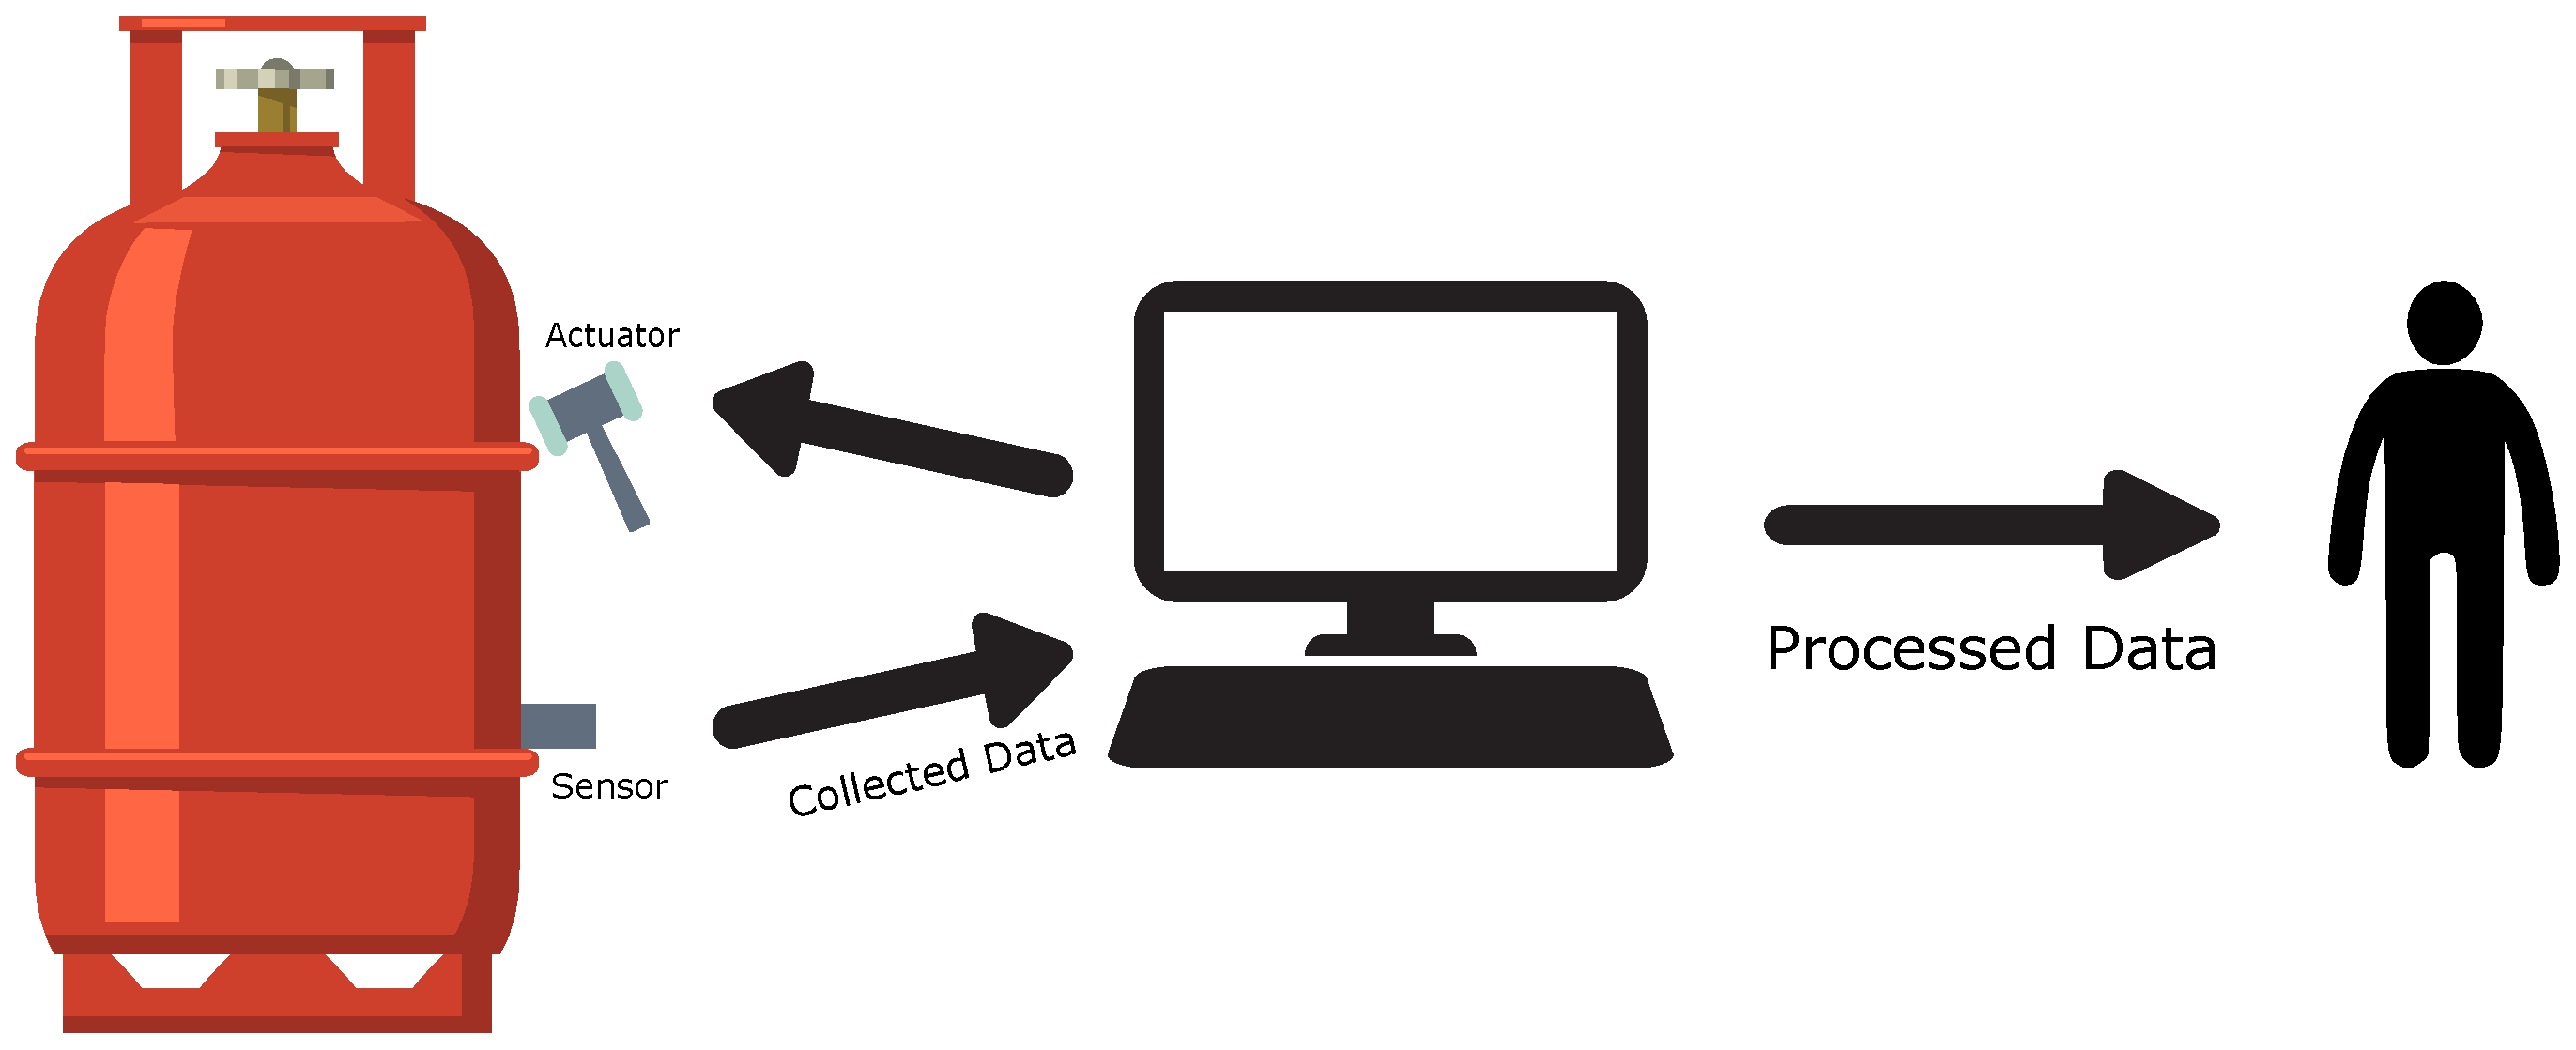
\includegraphics[width=0.55\textwidth]{Chapters/3CHP/Images/bottleBaseAct.eps}
    \caption{Basic architecture of the liquid level measuring device}{}
    \label{fig:systemArch}
\end{figure}
In the device, the processing unit is responsible for the control of the system as well, the unit is responsible for trigger the actuator in the first place, when this happens the hammer hits the side surface of the LPG bottle and thus the vibration is produce. In the mean time, the process unit starts to convert the signal from the sensor and store that value. Then the recorded data must be processed, in order to return to the user the desire information. Ideally, this procedure would occur once or twice a day, unless a manual measure was requested by the user, but for the purpose of the development of the device, the main purpose is to, in a first stage to get information and being able to associate the same information to the liquid level.

The chosen method to process the information, is throw the analysis of the acquired data in the frequency domain, for that a FFT is the chosen method to process the data and later be able to observe and associate the same information with the liquid level. A brief and visual description of the flow of how the process is suppose to occur in the processing unit is illustrated in figure~\ref{fig:systemSWFlow}.

\begin{figure}[]
    \centering
    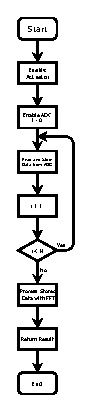
\includegraphics[width=0.15\textwidth]{Chapters/3CHP/Images/fluxogramArchProp.eps}
    \caption{Proposed diagram for the device operation}{}
    \label{fig:systemSWFlow}
\end{figure}
\todo[inline,color=red!40]{Should I explain the diagram, or isn't necessary from the explanation before the ilustration?}

\section{Problem Approach}
The approach to obtain a solution and hopefully a device capable of measuring correctly the LPG liquid level will be split in two main phases, each one of them with a different purpose, they are the study of behavior of the system to a external stimulation and the development of the solution for this case. In the two phases the Hardware selection will be different, but on the other hand to what concerns the data processing will be a mixture of different approaches.
In the first stage and in order to understand the behavior, limit the range of analysis of the data and define to the LPG bottle a maximum and minimum value of liquid, it will be used a hammer, a microphone and a computer installed with MatLab, this will allow to capture the sound produced when hitting the side surface of the LPG bottle, and process it in MatLab with the FFT function to analyze the spectrum of the acquired data.

The second stage will be divided in several smaller steps, so is possible to mislead any source of problems. In this stage the microphone will be replaced with two sensors, with the same purpose, in a first stage the hammer will continue to be used as a stimulation method, although later will be replaced with a solenoid, in order to perform automatically the trigger and the signal acquisition. In the same way, in the beginning MatLab will still be used to process the data, but later is to use a microcontroller for that purpose, although for capturing the signals from the sensors, a microcontroller will be used as the interface, and then send the data to the computer. The reason for this is that this way is easier to understand the type of signals acquired from the sensors and how is the proper way to process this data later, on a implementation, avoiding skipping steps.
\section{End of chapter considerations}
From the identification of the elements of the system, it is possible to define an approach to the problem presented, this chapter focuses exactly on that. Knowing those elements we are able to start to work in each element in order to integrate them in the final solution. The following two chapters will be dedicated to explore each element individually, they will be divided in two to separate the hardware/physical elements from the software.

\clearpage
%\printbibliography[heading=subbibliography]
%\addcontentsline{toc}{section}{References}